% thesis.tex
%
% This file is root file for an example thesis written using the
% IIT Guwahati LaTeX Style file.

% The IIT Guwahati LaTex Style is a modified
% version of IIT Bombay LaTex Style created by
% Dr. Amey Karkare (21 June 2007).
%
% Required permissions have been taken from Dr. Karkare in order to
% create the IIT Guwahati LaTex Style using his original work.
% Revision done by: Mandar Kulkarni, EEE Department, IIT Guwahati
% Further revised by Dr. Sonali Chouhan, EEE Department, IIT Guwahati (16/04/2016)

%=====================================================================
% Read: README.txt for more information
%=====================================================================

%=====================================================================
% DOCUMENT STYLE
%=====================================================================
% IITG Thesis format default settings are:
%   12pt, one-sided printing on a4 size paper
\documentclass{iitgthesis}
% For two-sided printing, with Chapter starting on odd-numbered pages,
% use the following line instead:
%%\documentclass[openright,twoside]{iitgthesis}

%=====================================================================
% OPTIONAL PACKAGES
%=====================================================================
% To include optional packages, use the \usepackage command.
% For e.g., The package epsfig is used to bring in the Encapsulated
%    PostScript figures into the document.
%    The package times is used to change the fonts to Times Roman;
%=====================================================================
\usepackage{epsfig}
\usepackage{stackrel}
\usepackage{epsf}
\usepackage{amssymb}
\usepackage{amsthm}
\usepackage{graphicx}
\usepackage[english]{babel}
\usepackage{mathrsfs}
%\usepackage{fancyhdr}
\usepackage{verbatim}
\usepackage{amsmath,amssymb}

\usepackage{cite}
\usepackage{multirow,tabularx}
\usepackage{ifthen}
% Add these after the document class declaration
\usepackage{times}
\DeclareMathAlphabet{\mathpzc}{OT1}{pzc}{m}{it}
\usepackage{tikz}
\usetikzlibrary{shapes.geometric, arrows}
\usepackage{subcaption}
\usepackage{smartdiagram}
%\usepackage[T1]{fontenc}
\usepackage{lmodern}
\linespread{1.3}
\usepackage{graphicx}
\graphicspath{ {./fig2/} }
\usepackage{float}
\usepackage{pgf}
\usetikzlibrary{arrows,automata}
%\usepackage[latin1]{inputenc}
\usepackage{verbatim}

\usepackage{amssymb}
%\usepackage{dsfont}
%\usepackage{stmaryrd}
\usepackage{amsmath}
\usepackage{mathrsfs}
\usepackage{enumitem}
\usepackage{scrextend}
%=====================================================================
%  Single counter for theorems and theorem-like environments:
%=====================================================================
\newtheorem{thm}{Theorem}[section]
\newtheorem{theorem}{{\bf Theorem}}
\newtheorem{lemma}{{Lemma}}
\newtheorem{proposition}[theorem]{Proposition}
\newtheorem{corollary}{{\bf Corollary}}
\newtheorem{result}{{\bf Result}}

%=====================================================================
% NEW COMMANDS DEFINED FOR A EASY TO READ CODE
% You are free to add your own set of new commands here
%
\newcommand{\brac}[1]{\left({#1}\right)}
\newcommand{\sbrac}[1]{\left[{#1}\right]}
\newcommand{\cbrac}[1]{\left\{{#1}\right\}}
\newcommand{\expc}[2][]{E_{#1}\left[{#2}\right]}

% End of Preamble, start of document
%

\begin{document}
%\renewcommand{\rmdefault}{cmr}
\renewcommand{\baselinestretch}{1.0}
\fontfamily{lmr}
%=====================================================================
% Include the prelude for Title page, abstract, table of contents, etc
% You need to modify it to contain your details
% prelude.tex
%   - titlepage
%   - dedication (optional)
%   - approval sheet
%   - course certificate
%   - table of contents, list of tables and list of figures
%   - nomenclature
%   - abstract
%============================================================================


\clearpage\pagenumbering{roman}  % This makes the page numbers Roman (i, ii, etc)


% TITLE PAGE
%   - define \title{} \author{} \date{}
\title{Design \& Implementation of Quantum Computing Immune Cryptography Processor}
%\author{Abhishek Agrawal \\ Souradip Pal}
\author{\hspace{-10mm}Abhishek Agrawal\hspace{8mm}Souradip Pal\\\hspace{-6mm}(150102002)\hspace{19mm}(150102076)}

%\authorone{Abhishek Agrawal}
%\authortwo{Souradip Pal}

\date{April 2019}

%  - Roll number, required for title page, approval sheet, and
%    certificate of course work
\rollnum{150102002\hspace{10mm}150102076}
%\rollnumone{150102002}
%\rollnumtwo{150102076}

%   - The default degree is ``Doctor of Philosophy''
%     (unless the document style msthesis is specified
%      and then the default degree is ``Master of Science'')
%     Degree can be changed using the command \iitbdegree{}
\iitgdegree{\textbf{Bachelor of Technology}}

%   - The default report type is preliminary report.
%      * for a PhD thesis, specify \thesis
\thesis
%      * for a M.Tech./M.Phil./M.Des./M.S. dissertation, specify \dissertation
%\dissertation
%      * for a DIIT/B.Tech./M.Sc.project report, specify \project
%\project
%      * for any other type, use  \reporttype{}
%\reporttype{project}

%   - The default department is ``Unknown Department''
%     The department can be changed using the command \department{}
\department{Department of Electronics \& Electrical Engineering}

%    - Set the guide's name
\setguide{Dr. Gaurav Trivedi}

%   - once the above are defined, use \maketitle to generate the titlepage
\maketitle

%--------------------------------------------------------------------%
% APPROVAL SHEET
%   - for final thesis, you need Approval Sheet. So, uncomment the
%     \makeapproval command.
%     it should come after dedication, if dedication is
%     present. Otherwise it is the first page after title page.
\makeapproval


%--------------------------------------------------------------------%
% COPYRIGHT PAGE
%   - To include a copyright page use \copyrightpage
% \copyrightpage

%--------------------------------------------------------------------%

% ACKNOWLEDGMENTS (optional)
%\begin{acknowledgments}
%Sample Acknowledgement
%\end{acknowledgments}


% ABSTRACT
\begin{abstract}

Recent advancements in the domain of Quantum Computing are posing a security threat to most of the classical cryptographic methods and algorithms. Most popular symmetric and asymmetric cryptosystems including RSA, ECC, DES, Diffie-Hellman etc. can be efficiently broken down by a quantum computer running Shor's Algorithm. There exist two methods to counter this threat: firstly using \textbf{Quantum Cryptography} which involves setting up a quantum channel, quantum computers and would require a complete overhaul of the data communication infrastructure. Second alternative called \textbf{Post-Quantum Cryptography}, can however be implemented on the existing infrastructure and is equally resistant to classical and quantum crypto-attacks. Post-Quantum Cryptographic algorithms are more immune to these attacks because they are designed on the weakness of quantum circuits and algorithms. Hash, Code, Lattice based and Multivariate Polynomial based cryptographic algorithms are the most popular class of such algorithms. {\em In this report, we present the design and hardware implementation of a chaos-based post-quantum cryptographic system derived from a mechanical model showing non-linear dynamics and show its resistance against quantum computing attacks.} We also provide in this report the details of the encryption-decryption algorithms and experimentations performed on the implementation of the system in {\em Artix FPGA} hardware platform. 

\end{abstract}


%--------------------------------------------------------------------%
% CONTENTS, TABLES, FIGURES
\tableofcontents
%\listoftables
\listoffigures

%--------------------------------------------------------------------%
% NOMENCLATURE
\begin{nomenclature}
\begin{description}
\item{\makebox[0.75in][l]{{FPGA}}} Field Programmable Gate Array

\item{\makebox[0.75in][l]{{DSA}}} Digital Signature Algorithm

\item{\makebox[0.75in][l]{{RSA}}} Rivest-Shamir-Adleman

\item{\makebox[0.75in][l]{{DES}}} Data Encryption Standard

\item{\makebox[0.75in][l]{{PQC}}} Post-Quantum Cryptography

\item{\makebox[0.75in][l]{{ECC}}} Elliptic Curve Cryptography

\item{\makebox[0.75in][l]{{NTRU}}} Nth-Degree Truncated Polynomial Ring

\item{\makebox[0.75in][l]{{ODE}}} Ordinary Differential Equation

\item{\makebox[0.75in][l]{{CLB}}} Configurable Logic Block

\item{\makebox[0.75in][l]{{ALU}}} Arithmetic Logic Unit

\item{\makebox[0.75in][l]{{LUT}}} Look-Up Table

\item{\makebox[0.75in][l]{{USB}}} Universal Serial Bus

\item{\makebox[0.75in][l]{{FSM}}} Finte State Machine

\item{\makebox[0.75in][l]{{HDL}}} Hardware Description Language

\item{\makebox[0.75in][l]{{RTL}}} Resistor Transfer Level
\end{description}
\end{nomenclature}

\cleardoublepage\pagenumbering{arabic} % Make the page numbers Arabic (1, 2, etc)


%=====================================================================
% Include the technical part of the report
\chapter{Introduction}
\label{chap:intro}
\setlength{\parskip}{1.5mm}
%\setlength{\baselineskip}{1.4mm}
\section{Motivation}
% Today, we send data from one computer to another without a second thought assuming a secure connection between them. But what if that connection cannot be trusted? The impact in the world economy can be devastating. E-commerce, cloud services, online stock trading and anything that relies that on the internet security would be rendered useless. This scenario is plausible in not too distant future. A developing technology called quantum computing would be able to break the encryption that is the backbone of secure internet communication. Today, secure communication relies on exchange of keys or secret codes to ensure parties are who they say they are and exchange messages that can't be read by others.

In this modern era, while transferring data from one computer to another, we almost everytime assume a secure connection. However, in a situation where this security is broken, the effects can be devastating and almost all the businesses and services relying on internet including banking and cloud services would be rendered useless. Such a situation may not be too distant in future. Advancements in quantum computing have posed a threat to the existing cryptographic methods on which the complete data communication infrastructure relies on, including the most popular public-key cryptography.

In 1994, a mathematician named Peter Shor, developed an algorithm which is able to break the security of key exchanges and digital signatures. Using this algorithm, a quantum computer would be able to crack the most sophisticated encryption in a matter of minutes. Quantum computers operate differently from traditional computers i.e. they work at atomic level. The essential units of a quantum computer is a qubit in contrast to bits used in traditional computers. A qubit is able to represent 0 and 1 simultaneously. Due to this property, few qubits can speed up certain types of computation by an enormous amount and hence quantum computers are more suitable for brute-force exhaustive searches. Although, this new technology is ideal for solving complex problems in astrophysics, pharmaceuticals and weather forecasting, it can also break the encryption and endanger our privacy and security.\\\\\\

\section{Problem Definition}
The objective of this project is to design and implement a chaos-based cryptographic system on hardware that is secure against Shor's Algorithm running on an ideal quantum computer.

This problem focuses on going beyond traditional cryptographic methods and implementing a new chaos based encryption-decryption technique in dedicated hardware like Field Programmable Gate Array (FPGA). Our aim is to design the system in such a way that it is simple enough to be implemented in practice, it is computationally efficient and it provides a reasonable degree of security. The system must also possess a number of fundamental features which are important for any cryptosystem in general. In order to achieve this goal some necessary steps to be performed along with the design and implementation are:
\begin{itemize}
  \item Verification of Encryption-Decryption Algorithm
    \begin{itemize}
        \item Validity of chaotic nature and quantum-safe properties of the scheme
    \end{itemize}

  \item Hardware-level optimization of the Algorithm
    \begin{itemize}
        \item Efficient pipelining of the algorithm for fast response in practical scenarios
    \end{itemize}
  \item Key Generation \& Management
    \begin{itemize}
        \item Storage and maintenanace of valid keys and efficient key exchange strategies
    \end{itemize}
  \item Security Analysis of the Cryptosystem
    \begin{itemize}
        \item Analysis of randomness and running time of the system
    \end{itemize}
\end{itemize}
        % Chapter 1: Introduction
\chapter{Preliminaries}
\label{chap:prelim}
%\setlength{\parskip}{1.5mm}
%\setlength{\baselineskip}{1.4mm}

\section{Present-day Cryptography}
Cryptography is the  study and practice of techniques for secure data transfer over insecure channels in presence of unauthorized users, usually called adversaries. Prior to modern age, cryptography was most exclusively referred to as encryption, i.e. the process of converting data from readable state to apparent noise.

Most of the present-day encryption algorithms are based on overlapping theory of mathematics and computer science. These are largely designed around `trap-door functions', i.e. problems with sufficient computational hardness. These problems can be theoretically solved, but is is not possible to do within reasonable time and with the resources that are usually at disposal.

Advances in mathematics such as improved algorithms on the integer factorization problem and discrete logarithm problem and availability of more computational power require these methods to adapt with time. Most of the algorithms can, however, be made secure against these advancements just by increasing the key-length.

\section{Shor's Algorithm}
Published in 1995 and named after it's formulator, Shor's algorithm, is a quantum algorithm for finding the prime factors of any given integer N.

The importance of Shor's algorithm lies in it's ability to find the prime factors of an integer in polynomial time, in comparison to the most efficient classical algorithms known, such as general number field sieve, which takes sub-exponential time. This is possible to due to efficiency of quantum fourier transform and modular exponentiation by repeated squaring.

\section{Shor's Algorithm \& Present Encryption Methods}
All of the popular cryptographic algorithms rely on one of the three hard problems - integer factorization problem, the discrete logarithm problem or the elliptic-curve discrete logarithm problem. These problems were viewed as important because many cryptography systems rely upon the difficulty of factoring large numbers. If an efficient method of factoring large numbers can be implemented, most of the encryption schemes would be next to worthless to protect their data. 

With Shor's algorithm, these can be be solved in reasonable polynomial time. This implies that, with a quantum computer having sufficient number of qubits, Shor's algorithm can be used to break the public-key cryptography schemes including RSA. However, the experimental quantum computers available today succumb to noise and decoherence problems, hence, cannot be used to break current encryption schemes.

\section{Post-Quantum Cryptography}
Post-Quantum Cryptography refers to the study of classical encryption schemes that are considered to be secure against an attack by quantum computers. As discussed above, most of the popular encryption methods can be efficiently broken using a sufficiently powerful hypothetical quantum computer. Thus, scientists are preparing methods to secure data against attacks when quantum computing becomes much more powerful.

Daniel J. Bernstein[11] lists the following important classes of cryptographic methods beyond RSA, DSA and ECRSA -
\begin{description}[align=left, style=multiline,leftmargin=4 cm]
\item [Hash-based - ] This includes Merkle's hash-tree public-key signature system, building upon the one-message idea.
\item [Code-based - ] An example is McEliece's hidden-Goppa-code public-key encryption system.
\item [Lattice-based - ] The most popular example that garnered most of the interest is Hoffstein-Pipher-Silverman NTRU public-key-encryption system.
\item [Multivariate quadratic equation based- ] One of the examples is Patarin's {\em HFEv} public-key-signature system originally proposed by Matsumoto and Imai.\\
\item [Secret-key based - ] The prominent example is the DaemenRijmen
{\em Rijndael} cipher which was later named AES (Advanced Encryption Standard).
\end{description}

\begin{figure}[H]
\centering
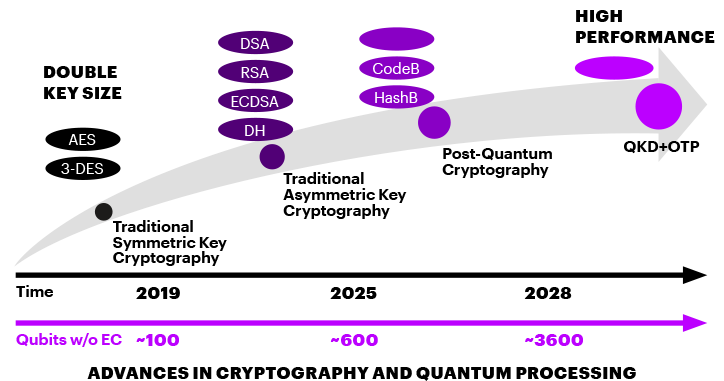
\includegraphics[width=14cm]{timeline.png}
\caption{Timeline for Cryptography \& Quantum Processing}\label{fig:timeline}
\end{figure}


%All of these encryption methods are considered to be resistant to both classical and %quantum computing. These schemes are built around cryptographic primitives for which no %efficient algorithm has been found yet, either for quantum or for classical computers.


\section{Chaos based Cryptography}
Apart from the popular post-quantum cryptographic methods, a new method of constructing cryptosystems utilising the non-predictability property of discrete chaotic systems has become somewhat noteworthy from practical perspectives. This type of systems are based on the characteristics of chaos, which are sensitivity of parameters, sensitivity of initial points, and randomness of sequences obtained by iterating a chaotic map. A ciphertext is obtained by the iteration of an inverse chaotic map from an initial point denoting a plaintext. 

If the number of iterations is large enough, the randomness of the encryption and the decryption functions would be so large that attackers would be unable to break this cryptosystem by statistical characteristics. Hence, nonlinear dynamic systems with chaos are generally viewed to be good candidates for constructing such encryption-decryption algorithms. Most of these methods have been used in the development of symmetric ciphers for encryption of 2D images.

\begin{figure}[H]
\begin{subfigure}{0.5\textwidth}
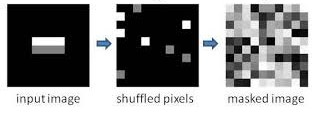
\includegraphics[width=1\linewidth]{image_chaos0.jpg}
\caption{Image Encryption using 1D Chaotic Map}\label{fig:image_chaos0}
\end{subfigure}
\begin{subfigure}{0.5\textwidth}
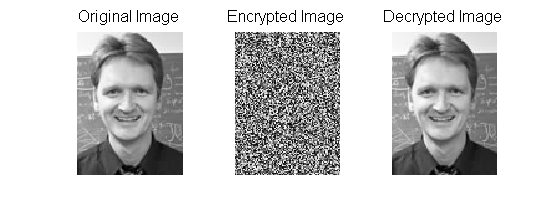
\includegraphics[width=1\linewidth]{image_chaos.png}
\caption{Chaos based Image Encryption}\label{fig:image_chaos}
\end{subfigure}
\caption{Chaos based Cryptography}\label{fig:image0}
\end{figure}

\section{Field Programmable Gate Array}
A field programmable gate array is a set (array) of reconfigurable gates that can implement both sequential and combinational logic including multi-level logic functions.

FPGAs are built in form of an array of configurable logic blocks (CLBs). Each of these CLBs can be programmed to perform a logic function and then connected to each other through a hierarchy of interconnects (routing channels) to form a complex logic. FPGA also has a set of I/O elements for interfacing with external devices such as flash memories and network ports.

The structure of CLBs varies with model and manufacturers, but all of them share a lot of similarity. Figure 2.3 shows the structure of Cyclone IV CLB, consisting of a 4-input LUT and a flip-flop. By loading appropriate values, the LUT can be programmed to perform any 4-input function. Further, the choice of multiplexer select signals determines how the data is routed through LUT to the neighbouring LEs and IOEs. The LUT output either goes directly to the LE output for combinational logic, or it can be routed through the register for sequential logic.
\begin{figure}[H]
\centering
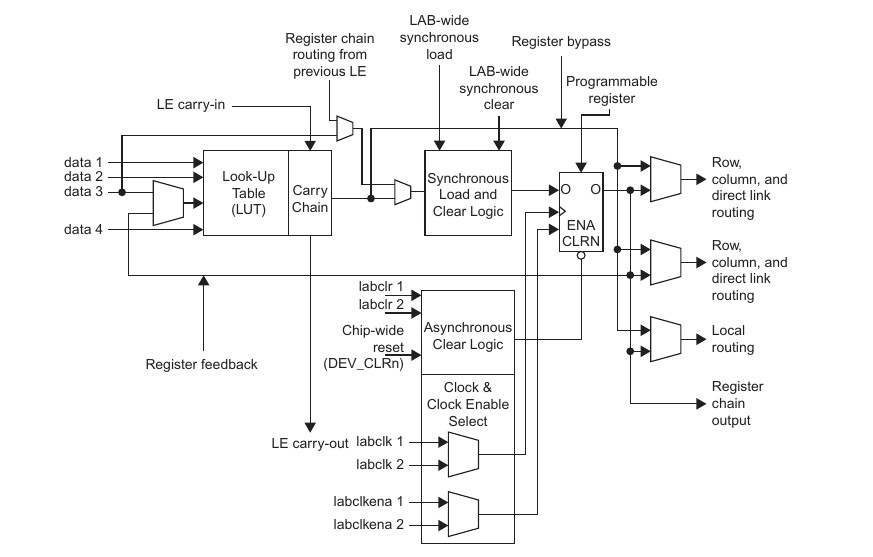
\includegraphics[width=13cm]{fpga.jpg}
\caption{FPGA CLB Structure}\label{fig:fpga}
\end{figure}

An engineer programs the logic using Hardware Description Language (HDLs) such as VHDL or Verilog. A synthesis is then used to generate a gate-level netlist. An implementation tool then determines how the CLBs and routing channels should be configured to perform the specified function and generates a bitstream that can be loaded into a FPGA.
       % Chapter 2: Introduction
\chapter{Literature Survey}
\label{chap:lit}
\setlength{\parskip}{1.5mm}
%\setlength{\baselineskip}{1.4mm}
\section{Chaos and Cryptography}
Over last few years, there has been a great interest in understanding the working of chaotic systems. They are distinguished by their high sensitivity to initial conditions, statistically similar to random signals and a continuous broad-band power spectrum. This has garnered interest from cryptanalysts and there have been several publications proposing various chaos-based cryptographic systems such as in [2], [3].

The chaos-based cryptosystems can be sub-divided into two classes. First one involves numerically computing a large number of iterations over time of a chaotic system, using message as the initial data. (see [5], [6]). The second class amounts to scrambling a message with a chaotic dynamic. This includes additive masking, chaotic switching, message embedding, etc.

The relevance and usefulness of chaos in these systems have been demonstrated through comparative studies between characteristics of chaotic systems and requirements of a strong cipher (see [1], [4]). Several properties of chaotic maps are similar to those of cryptographic maps : extreme sensitivity to initial conditions and parameters, unstable periodic orbits with large time-periods. Further, iterations of chaotic map spread the initial region over entire map, introducing diffusion which is an important requirement for a strong cipher.

\section{Discrete Chaos}
It must be noted that when chaotic systems are simulated on computers with limited precision, the sequences x\textsubscript{k} generated are not exactly chaotic. Since, the cardinality of this set is finite, such sequences will always be a part of a loop of finite period. It can be expected that this period wouldn't be too short and will be greatly chaotic in nature. Claiming such properties, however, requires some consideration [7]. Contributions made in this regard and discussion about discrete chaos can be found in [8]. However, some noteworthy takeaways are listed below -
\begin{itemize}
\item Through numerical experiments, it has been shown that mean cycle L of such a system is O(2\textsuperscript{P/2}), where P is the amount of precision in terms of number of bits. This serves as good reference while working with chaotic systems. However, it must be verified as there are no mathematical proofs to support it.
\item The rounding error in computer systems poses another problem. The errors made in each iteration will culminate at a very fast rate due to high sensitivity of the system on the initial conditions. Thus, the actual trajectory and the calculated trajectory will be considerably different after a few iterations. However, "Shadowing Lemma" in [10], guarantees that one can always find an actual trajectory that is arbitrarily near the calculated trajectory.
\end{itemize}

\section{Chaos in Non-Linear Dynamic Systems}
Many real world phenomena can be mathematically modelled as non-linear dynamic systems. Out of these phenomena, some exhibit significant degree of chaos. The unpredictability of these non-linear phenomena is due to the fact that the system passes through a series of {\em unstable states}. Also, these non-linear systems generally display very sensitive dependence on initial conditions which is the main reason for generating chaotic maps using non-linear dynamic systems. It must, however, be noted that not every complicated dynamic behavior can be considered chaotic. Chaotic systems differ from {\em noisy motion} in that their randomness is due to interaction of few simple laws. The quantitive description, however, lies in the concept of Lyapunov exponents which measures the exponential divergence of trajectories of the chaotic maps. 

\section{Baptista-type Cryptosystem}
Proposed by M.S. Baptista, this is a chaotic-cryptosystem based on the interval partitioning of chaotic orbits of the logistic map. This uses the ergodic property of chaos, which enables the construction of fast and secure chaotic encryption-decryption schemes due to its simplicity and
less complex structure. The main idea of this scheme is to first map the text characters to real values and then algorithms are applied to
encrypt the message. Decryption is performed by iterating the chaotic map and then corresponding symbol for the real values are obtained.

          % Chapter 3: Literature survey
\chapter{Proposed Approach}
\label{chap:system}
\setlength{\parskip}{1.5mm}
%\setlength{\baselineskip}{1.4mm}
The proposed algorithm of encryption \& decryption is based on multiple iterations of a certain dynamical chaotic system and using a Baptista-type encryption-decryption scheme from the chaotic map generated. After referring extensive literature and keeping in mind the resources at our disposal, we have decided to take the compound triple-pendulum model for creating the chaotic map in our cryptosystem. We assume that input to the system is a plain message. The system parameter(s) and additionally the initial conditions of the dynamical system are assumed to be the part of the secret key. After simulating the triple-pendulum, our next step would be to generate a valid set of keys for encryption and decryption. The entire mechanical model would then be implemented on {\em Artix FPGA} including the design and implementation of ALU and Control Unit, adhering to the performance specification of the problem. Additionally, an extra data transfer module can be added to the hardware for key exchanges.\\
The entire approach can be summarized using the following roadmap :- 
\begin{figure}[H]
\vfill
\tikzstyle{startstop} = [rectangle, rounded corners, minimum width=3cm, minimum height=0.8cm,text centered, draw=black, fill=orange!30]
\hspace{1.8cm}
\begin{tikzpicture}[node distance=1.1cm]

\node (block1) [startstop, yshift=-4cm] {Choosing an encryption strategy based on Chaotic Map};

\node (block2) [startstop, below of=block1] {Simulation of Triple-Pendulum using State-Space Method};

\node (block3) [startstop, below of=block2] {Generating a set of Valid Keys};

\node (block4) [startstop, below of=block3] {Parallelization of algorithm for FPGA implementation};

\node (block5) [startstop, below of=block4] {Implementation of Encryption-Decryption scheme into an FPGA};

\node (block6) [startstop, below of=block5] {Designing variable-precision ALU \& Control Unit};

\node (block7) [startstop, below of=block6] {Adding Ethernet and USB functionality for data transfer};

\draw [->] (block1) -- (block2);
\draw [->] (block2) -- (block3);
\draw [->] (block3) -- (block4);
\draw [->] (block4) -- (block5);
\draw [->] (block5) -- (block6);
\draw [->] (block6) -- (block7);
\end{tikzpicture}
\vfill
\caption{Implementation Steps}
\end{figure}
              % Chapter 4: System model and formulating the problem statement
\chapter{Work Progress}
\label{chap:work}
\setlength{\parskip}{1.5mm}
%\setlength{\baselineskip}{1.4mm}
\section{Verifying the Algorithm in MATLAB}
\subsection{Model of Non-Linear Dynamic System}
A schematic diagram of the compound triple-pendulum system is shown in Figure 5.1.The bars of the pendulum have significant mass so that it can be modeled as a compound pendulum. The model has been parameterized according to the physical characteristics of the system including mass of the bars, their inertia etc. 
% Damping factors were also included in the model for higher degree of chaos and non-linearity in the system. 
% Each bar ${i}$ is defined by a set of four parameters: 
% ${I_{i}}$, the moment of inertia of the bar, ${m_{i}}$, the mass of the bar,
%  ${L_{i}}$, the length of the bar, and
%  ${k_{i}}$, the damping coefficient of the bar rotating about it’s upper joint. 
The position and velocity of the bars are defined by the six system state variables: $\theta$\textsubscript{1}, $\theta$\textsubscript{2}, $\theta$\textsubscript{3}, ${\dot{\theta\textsubscript{1}}}$, ${\dot{\theta\textsubscript{2}}}$, ${\dot{\theta\textsubscript{3}}}$

%\begin{figure}
%\centering
%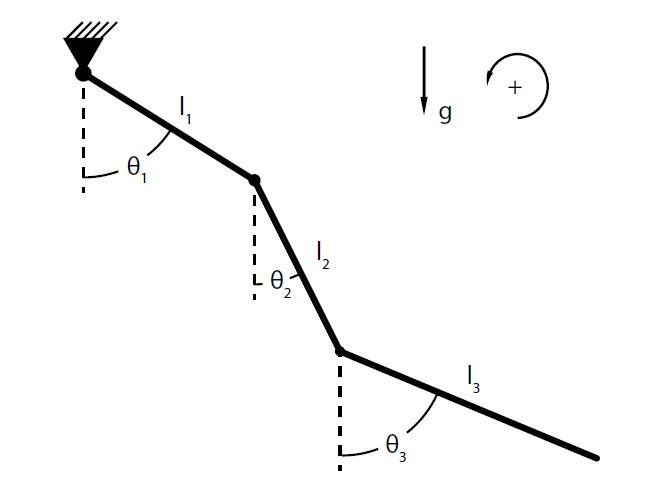
\includegraphics[width=8cm]{pendulum.jpg}
%\caption{Schematic Diagram of Triple Pendulum System}\label{fig:pendulum}
%\end{figure}
% 

\begin{figure}[H]
\begin{subfigure}{0.5\textwidth}
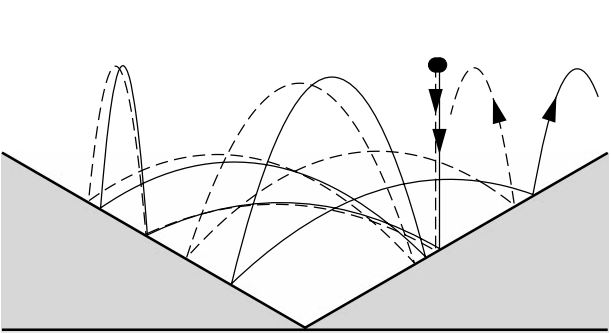
\includegraphics[width=1.1\linewidth]{ball.jpg}
\caption{Chaotic motion of a bouncing ball}\label{fig:ball}
\end{subfigure}
\begin{subfigure}{0.5\textwidth}
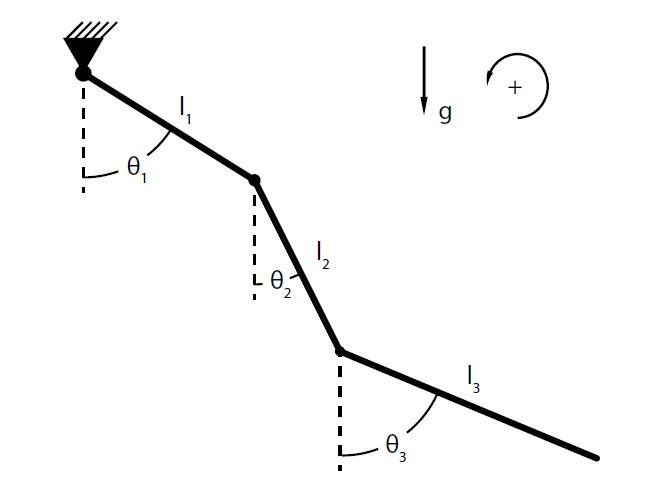
\includegraphics[width=0.8\linewidth]{pendulum.jpg}
\caption{Schematic Diagram of Triple Pendulum}\label{fig:pendulum}
\end{subfigure}
\caption{Examples of Non-Linear Dynamic systems}\label{fig:image1}

\end{figure}
\begin{figure}[h]
\begin{subfigure}{0.5\textwidth}
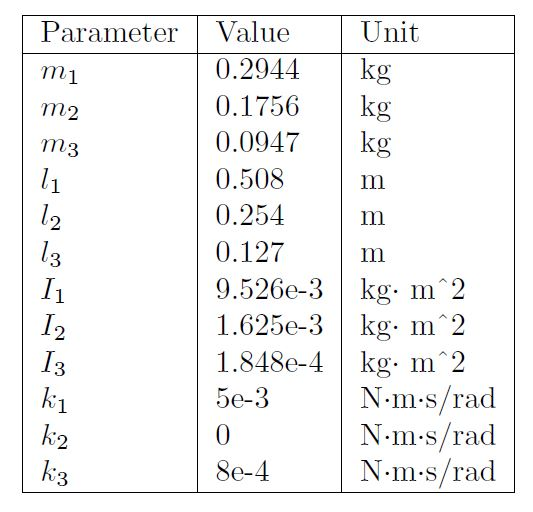
\includegraphics[width=0.8\linewidth]{param.jpg}
\caption{Table 1}\label{fig:param}
\end{subfigure}
\begin{subfigure}{0.5\textwidth}
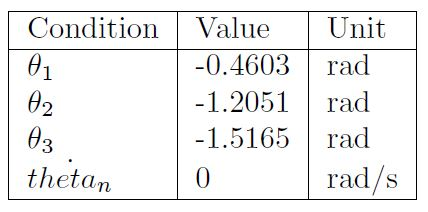
\includegraphics[width=0.8\linewidth]{ic.jpg}
\caption{Table 2}\label{fig:ic}
\end{subfigure}
\caption{Parameters \& Initial Conditions for the Initial Value Problem}\label{fig:image2}
\end{figure}

% \begin{figure}
% 
% 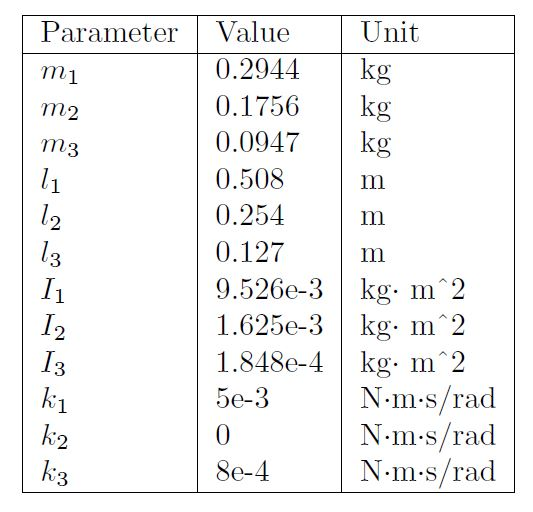
\includegraphics[width=8cm]{param.jpg}
% \caption{Parametric Values used for Simulation}\label{fig:param}
% \end{figure}
% 
% \begin{figure}
% % \centering
% 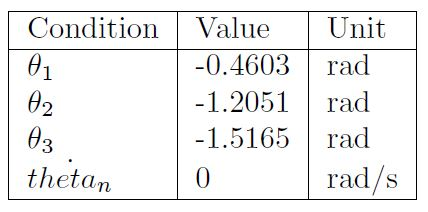
\includegraphics[width=8cm]{ic.jpg}
% \caption{Initial Conditions used for Simulation}\label{fig:ic}
% \end{figure}

\subsection{Simulation of Compound Triple Pendulum}
This compound triple-pendulum model has been simulated using MATLAB using approximate differential equations describing the random motions. The parameters and initial conditions of the ODEs are given in Table 1 and Table 2 respectively. For the simulation, simple numerical methods were used to solve the differential equations and the values corresponding to the angular position of the bars were obtained within a certain duration of time with a predefined precision. This generates the mapping values for the encryption module. 

% \begin{figure}[H]
% \centering
% 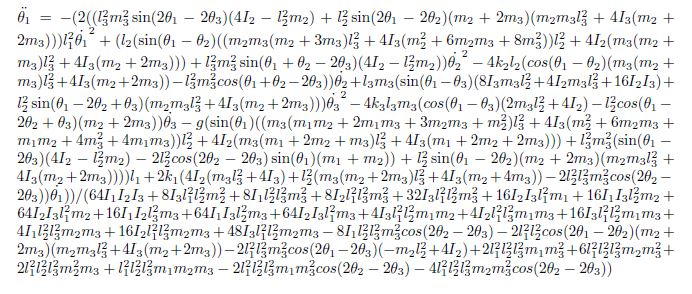
\includegraphics[width=16cm]{diff1.jpg}
% \caption{Differential Equation for ${\theta\textsubscript{1}}$}\label{fig:diff1}
% \end{figure}
% 
% 
% \begin{figure}[H]
% \centering
% 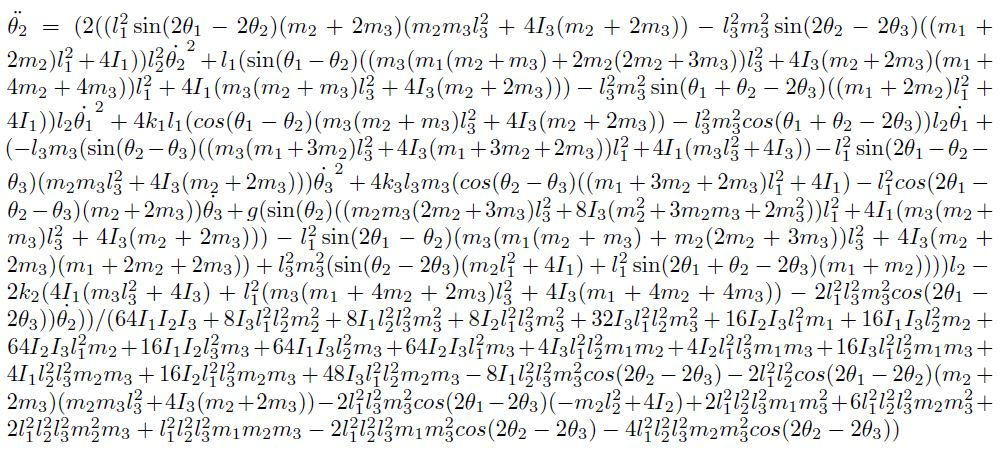
\includegraphics[width=16.5cm]{diff2.jpg}
% \caption{Differential Equation for ${\theta\textsubscript{2}}$}\label{fig:diff2}
% \end{figure}
% 
% 
% \begin{figure}[H]
% \centering
% 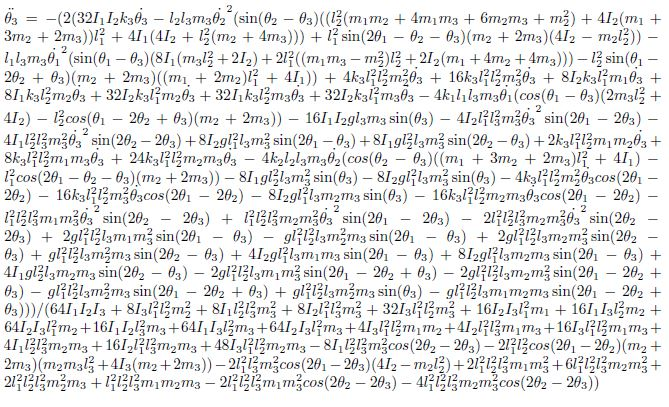
\includegraphics[width=16.5cm]{diff3.jpg}
% \caption{Differential Equation for ${\theta\textsubscript{3}}$}\label{fig:diff3}
% \end{figure}
% \vfill
\subsubsection{Simulation Results}
These are some of the observations from the simulation of the triple-pendulum model for a duration of t = 0 to t = 10 seconds with $\Delta$t = 0.001 :\\
(i) Initial conditions are same as given in Table 1 \& 2:\\
 
\begin{figure}[H]
\begin{subfigure}{0.5\textwidth}
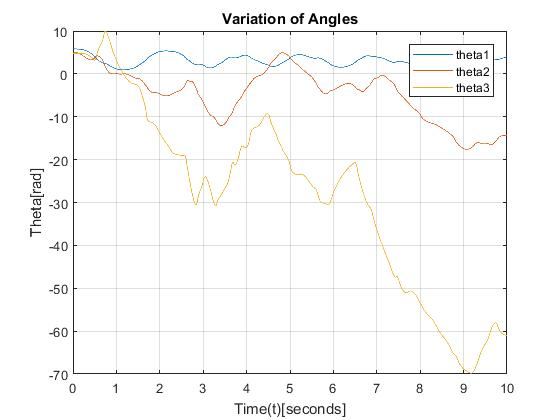
\includegraphics[width=1\linewidth]{theta.jpg}
\caption{Plot of ${\theta}$ vs Time}\label{fig:theta}
\end{subfigure}
\begin{subfigure}{0.5\textwidth}
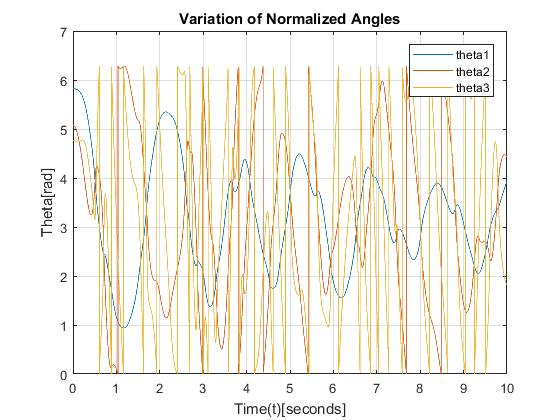
\includegraphics[width=1\linewidth]{theta_norm.jpg}
\caption{Plot of Normalized ${\theta}$ vs Time}\label{fig:theta_norm}
\end{subfigure}
\caption{Motion of Triple-Pendulum for t = 0 to t = 10 sec}\label{fig:image3}
\end{figure}

\begin{figure}[H]
\centering
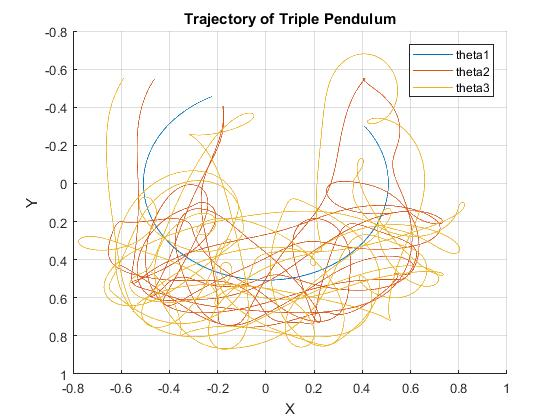
\includegraphics[width=0.7\linewidth]{trajectory.jpg}
\caption{Plot of Motion of Triple-Pendulum}\label{fig:trajectory}
\end{figure}


\subsection{Encryption - Decryption}
Our approach is to convert the plain-text into ascii format and  map the value to the partitioned intervals of the triple-pendulum motion simulated within a specific duration of time for a particular set of parameters and initial conditions. The initial conditions and parameters of the different equation forms a part of the private key. Following the Baptista-type method, the entire range of the chaotic function was partitioned into a number of intervals equal to the number of characters. Each character in the plain-text is then mapped to a specific interval and then to a time point randomly selecting from that interval.  

\begin{figure}[H]
\centering
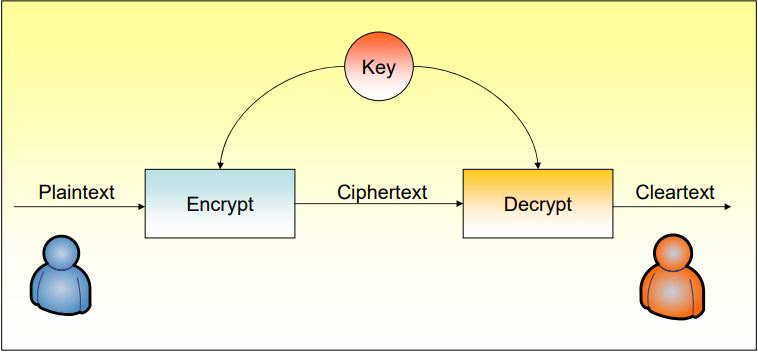
\includegraphics[width=10cm]{crypto.jpg}
\caption{Working Principle of a Symmetric Cryptosystem}\label{fig:crypto}
\end{figure}

On the decryption module, the interval in which the encrypted value lies is computed from the generated motion of the triple-pendulum for the same key and the corresponding index would then refer to the ascii converted clear-text. Converting them into characters, the message can be decoded.\\
\begin{figure}[H]
\centering
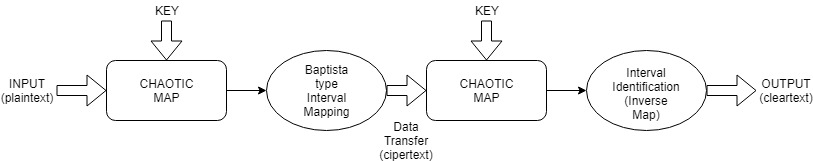
\includegraphics[width=16cm]{Dataflow.jpg}
\caption{Encryption-Decryption Strategy}\label{fig:Dataflow}
\end{figure}


\section{Key Generation}
It is observed that for certain specific parameters or initial conditions, the motion of the bars of the triple-pendulum shows periodic nature after a certain span of time. Hence there is a need to eliminate those parameters or initial conditions for which the motion is periodic as the periodic nature breaks the chaotic behavior of the system. For that a test for periodicity was employed to extract the prominent period of the signal using statistical analysis on the spectrum of the signal. The test used is known as {\bf{\em Fisher's g-statistic test}}(see [11]). This method is based on the test of significance of the periodic components of the signal derived from its periodogram. 

\begin{figure}[H]
\centering
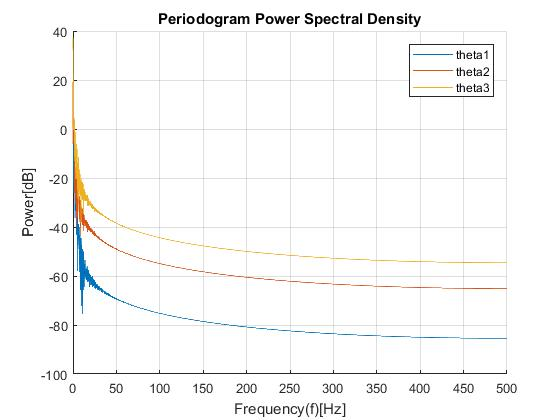
\includegraphics[width=0.7\linewidth]{periodogram.jpg}
\caption{Periodogram Plot for ${\theta}$}\label{fig:periodogram}
\end{figure}


\begin{figure}[H]
\begin{subfigure}{0.5\textwidth}
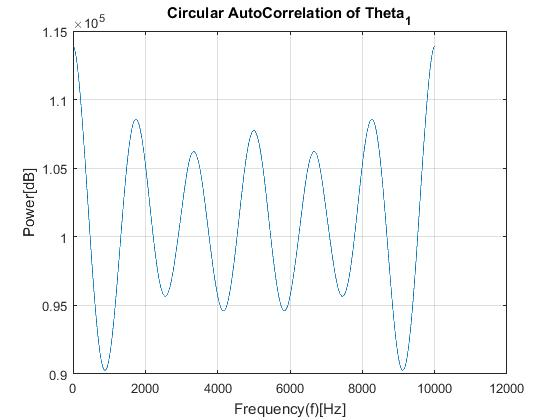
\includegraphics[width=1\linewidth]{auto_corr1.jpg}
\caption{Plot of Circular Auto-Correlation for ${\theta_{1}}$}\label{fig:cir_auto1}
\end{subfigure}
\begin{subfigure}{0.5\textwidth}
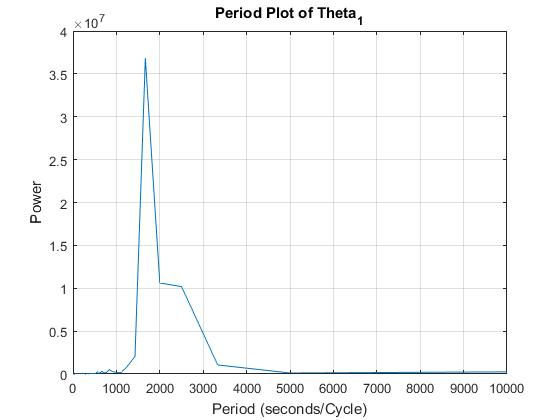
\includegraphics[width=1\linewidth]{period1.jpg}
\caption{Plot of Periodicity for ${\theta_{1}}$}\label{fig:period1}
\end{subfigure}
\caption{Periodic Properties of ${\theta_{1}}$}\label{fig:image4}
\end{figure}

\begin{figure}[H]
\begin{subfigure}{0.5\textwidth}
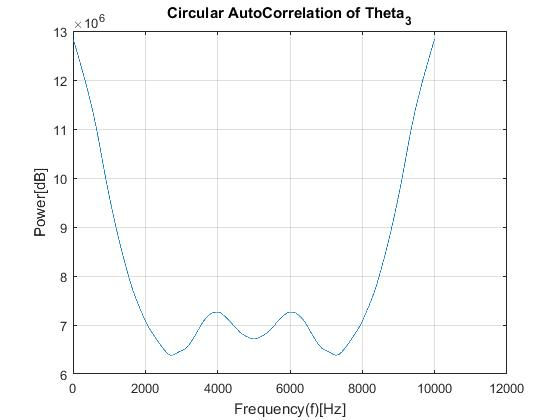
\includegraphics[width=1\linewidth]{auto_corr3.jpg}
\caption{Plot of Circular Auto-Correlation for ${\theta_{3}}$}\label{fig:cir_auto3}
\end{subfigure}
\begin{subfigure}{0.5\textwidth}
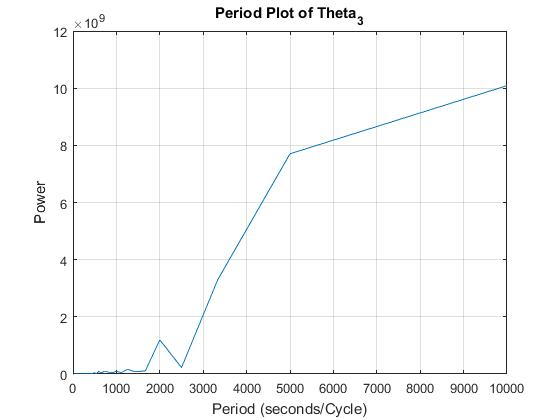
\includegraphics[width=1\linewidth]{period3.jpg}
\caption{Plot of Periodicity for ${\theta_{3}}$}\label{fig:period3}
\end{subfigure}
\caption{Periodic Properties of ${\theta_{3}}$}\label{fig:image5}
\end{figure}

From the figures 5.8 \& 5.9 , it is observed that there is peak at 1700 (seconds/Cycle) for $\theta_{1}$ whereas no such peak occurs for $\theta_{3}$. Thus $\theta_{1}$ is periodic in nature. The values obtained from the periodicity test and plots of circular auto-correlation clearly differentiates the parameters and initial values which leads to periodic nature of the motion and those which lead to non-periodic nature of the motion. Thus by iterating through all possibles values of the parameters and checking likewise for non-periodic nature, a set of keys was generated and stored. 


\section{FPGA Implementation}
The complete design is being implemented at Register-Transfer Level (RTL) in {\bf Verilog HDL} and the target device chosen is Digilent Nexys Board with {\bf Xilinx Artix-7 FPGA}. The following diagram shows the implementation plan for the design :
\begin{figure}[H]
\centering
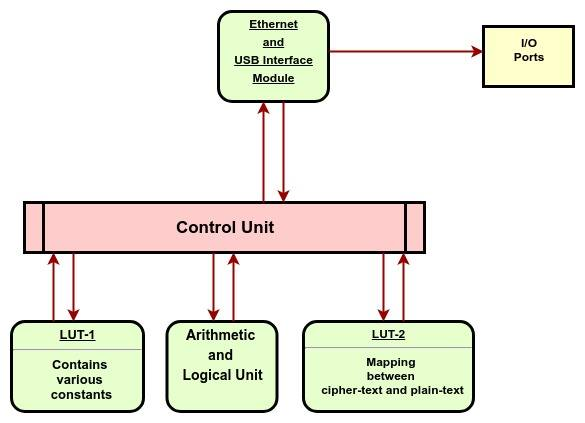
\includegraphics[width=10cm]{fpga_block.jpg}
\caption{Block Diagram of FPGA Implementation}\label{fig:fpga_block}
\end{figure}

1. {\bf Arithmetic and Logical Unit (ALU)} - The ALU uses floating-point arithmetic whose precision can be configured at the time of synthesis. This has been done to enable the study of how security strength varies with arithmetic precision.

2. {\bf Look-Up Table (LUT)} - A fast Look-Up table is to be implemented for storing various constants and the mapping between clear-text and cipher-text.

3. {\bf Ethernet and USB Module} - These are required to enable the device to encrypt or decrypt both a stream of data as well as complete file.

4. {\bf Control Unit} - Essentially a state machine that co-ordinates the operation of all other modules including evaluation of state-variables and transfer of data through USB/Ethernet port.

\section{Analysis}
\subsection{General Properties of the Cryptosystem}
\subsubsection{Test for Chaos}
There are some essential requirements that need to be obeyed by any chaos based cryptosystem. These requirements include:
\begin{enumerate}
	\item Sensitivity to Parametric values: A small variation in one of the system parameters is enough to make two trajectories, starting at the same initial point, separate at exponential rate.
	\item Sensitivity to Initial  Condition:  two  trajectories  starting  at  two  different,  though  arbitrarily  close,  initial points separate from each other exponentially.
	\item Ergodicity:  Almost every trajectory tends to an invariant distribution that is independent of the initial conditions, and almost every trajectory will eventually visit any arbitrary interval of arbitrary size.
\end{enumerate}

The proposed cryptosystem also holds such properties.The three qualities mentioned earlier are clearly evident from the plots and graphs shown Fig. ,Fig. \& Fig. . It is observed that keeping the parameters in one case and initial conditions in another case, constant leads to two completely different trajectories. Thus the map generated from the compound triple pendulum model possesses the essential chaotic properties to be employed in a general cryptosystem. 

\subsubsection{Collision Test}
Collision resistance is a property of cryptographic algorithms which makes it difficult to find two inputs which are encrypted to the same output. It must be ensured that finding collisions must be kept as hard as some of the hard mathematical problems like integer factorization  or discrete logarithm. Collision resistance does not mean that no collisions exist; simply that they are hard to find. Here, we show that the proposed algorithm is fully collision resistant i.e. no collisions exist.

Since the entire range of $\theta$'s are partitioned according to the number of characters(say 256), different characters are mappped to points in different intervals. Hence two different inputs having different characters are completely mapped to different intervals. So the encryption scheme is completely free of collisions. 

\subsubsection{Test for Randomness}
For testing randomness of the chaotic map, statistical tests are generally applied. These statistical tests are generally employed for testing randomness in pseudo random number generators. Here, Diehard random number generator test suite has been employed to do such tests. Developed by George Marsaglia, Diehard is a battery of tests which are used to determine the quality of PRNGs. The list of tests performed on the generated chaotic map data and the corresponding results obtained are shown in Table 5.1.

\begin{table}[h!]
\begin{center}
\caption{Dieharder Test}
\label{tab:table1}
\begin{tabular}{|c|c|c|c|c|c|} % <-- Alignments: 1st column left, 2nd middle and 3rd right, with vertical lines in between
    \hline
    \textbf{test\_name} & \textbf{ntup} & \textbf{tsamples} & \textbf{psamples} & \textbf{p-value} & \textbf{Assessment}\\
    \hline
    diehard\_birthdays &    0 &        100 &      100 & 0.98409924 &   PASSED \\  
    diehard\_operm5 &    0 &    1000000 &      100 & 0.02570841 &   PASSED \\  
    diehard\_rank\_32x32 &    0 &      40000 &      100 & 0.30314396 &   PASSED \\  
    diehard\_rank\_6x8 &    0 &     100000 &      100 & 0.07586247 &   PASSED \\  
    diehard\_bitstream &    0 &    2097152 &      100 & 0.83264505 &   PASSED \\  
    diehard\_opso &    0 &    2097152 &      100 & 0.93701062 &   PASSED \\  
    diehard\_oqso &    0 &    2097152 &      100 & 0.63759752 &   PASSED \\  
    diehard\_dna &    0 &    2097152 &      100 & 0.73795350 &   PASSED \\  
    diehard\_count\_1s\_str &    0 &     256000 &      100 & 0.77268562 &   PASSED \\  
    diehard\_count\_1s\_byt &    0 &     256000 &      100 & 0.55542008 &   PASSED \\  
    diehard\_parking\_lot &    0 &      12000 &      100 & 0.70977074 &   PASSED \\  
    diehard\_2dsphere &    2 &       8000 &      100 & 0.58428028 &   PASSED \\  
    diehard\_3dsphere &    3 &       4000 &      100 & 0.86446205 &   PASSED \\  
    diehard\_squeeze &    0 &     100000 &      100 & 0.19422339 &   PASSED \\  
    diehard\_sums &    0 &        100 &      100 & 0.33263813 &   PASSED \\  
    diehard\_runs &    0 &     100000 &      100 & 0.50609448 &   PASSED \\    
    diehard\_craps &    0 &     200000 &      100 & 0.36377661 &   PASSED \\   
    marsaglia\_tsang\_gcd &    0 &   10000000 &      100 & 0.66121444 &   PASSED \\ 
    sts\_monobit &    1 &     100000 &      100 & 0.31074688 &   PASSED \\  
    sts\_runs &    2 &     100000 &      100 & 0.98606705 &   PASSED \\  
    sts\_serial &    1 &     100000 &      100 & 0.23629469 &   PASSED \\  
    sts\_serial &    2 &     100000 &      100 & 0.85410639 &   PASSED \\  
    sts\_serial &    8 &     100000 &      100 & 0.11131795 &   PASSED \\  
    sts\_serial &   16 &     100000 &      100 & 0.83380616 &   PASSED \\  
    rgb\_bitdist &    1 &     100000 &      100 & 0.45061356 &   PASSED \\  
    rgb\_bitdist &    6 &     100000 &      100 & 0.53111009 &   PASSED \\   
    rgb\_bitdist &   12 &     100000 &      100 & 0.64865649 &   PASSED \\  
    rgb\_minimum\_distance &    2 &      10000 &     1000 & 0.41755433 &   PASSED \\   
    rgb\_minimum\_distance &    4 &      10000 &     1000 & 0.11298477 &   PASSED \\  
    rgb\_permutations &    2 &     100000 &      100 & 0.79654377 &   PASSED \\ 
    rgb\_permutations &    4 &     100000 &      100 & 0.85371565 &   PASSED \\  
    rgb\_lagged\_sum &    0 &    1000000 &      100 & 0.92039997 &   PASSED \\   
    rgb\_lagged\_sum &   16 &    1000000 &      100 & 0.78219023 &   PASSED \\   
    rgb\_lagged\_sum &   32 &    1000000 &      100 & 0.64955712 &   PASSED \\  
    rgb\_kstest\_test &    0 &      10000 &     1000 & 0.58005862 &   PASSED \\  
    dab\_bytedistrib &    0 &   51200000 &        1 & 0.01089458 &   PASSED \\  
    dab\_dct &  256 &      50000 &        1 & 0.06122408 &   PASSED \\  
    dab\_filltree &   32 &   15000000 &        1 & 0.12524761 &   PASSED \\   
    dab\_filltree2 &    0 &    5000000 &        1 & 0.50605989 &   PASSED \\  
    dab\_monobit2 &   12 &   65000000 &        1 & 0.27940682 &   PASSED \\  
        
    \hline
\end{tabular}
\end{center}
\end{table}

It is observed that in most of the tests, the chaotic map generator performs well. This can be attributed largely due to the non-linear dynamics of the map.\\\\

\subsection{Complexity}

In this report, we give an overview of the computational complexity of the algorithm both on software as well as hardware level.
           % Chapter 4: Analysis
\chapter{Results \& Conclusion}
\label{chap:conclusion}
\setlength{\parskip}{1.5mm}
%\setlength{\baselineskip}{1.4mm}

The entire top level module was simulated in Xilinx Vivado and the synthesis and working of each of the modules were verified. The functions of encryption \& decryption are also properly analysed. The results obtained in the hardware simulation matches with that simulated in MATLAB within some reasonable accuracy.

\begin{figure}[H]
\centering
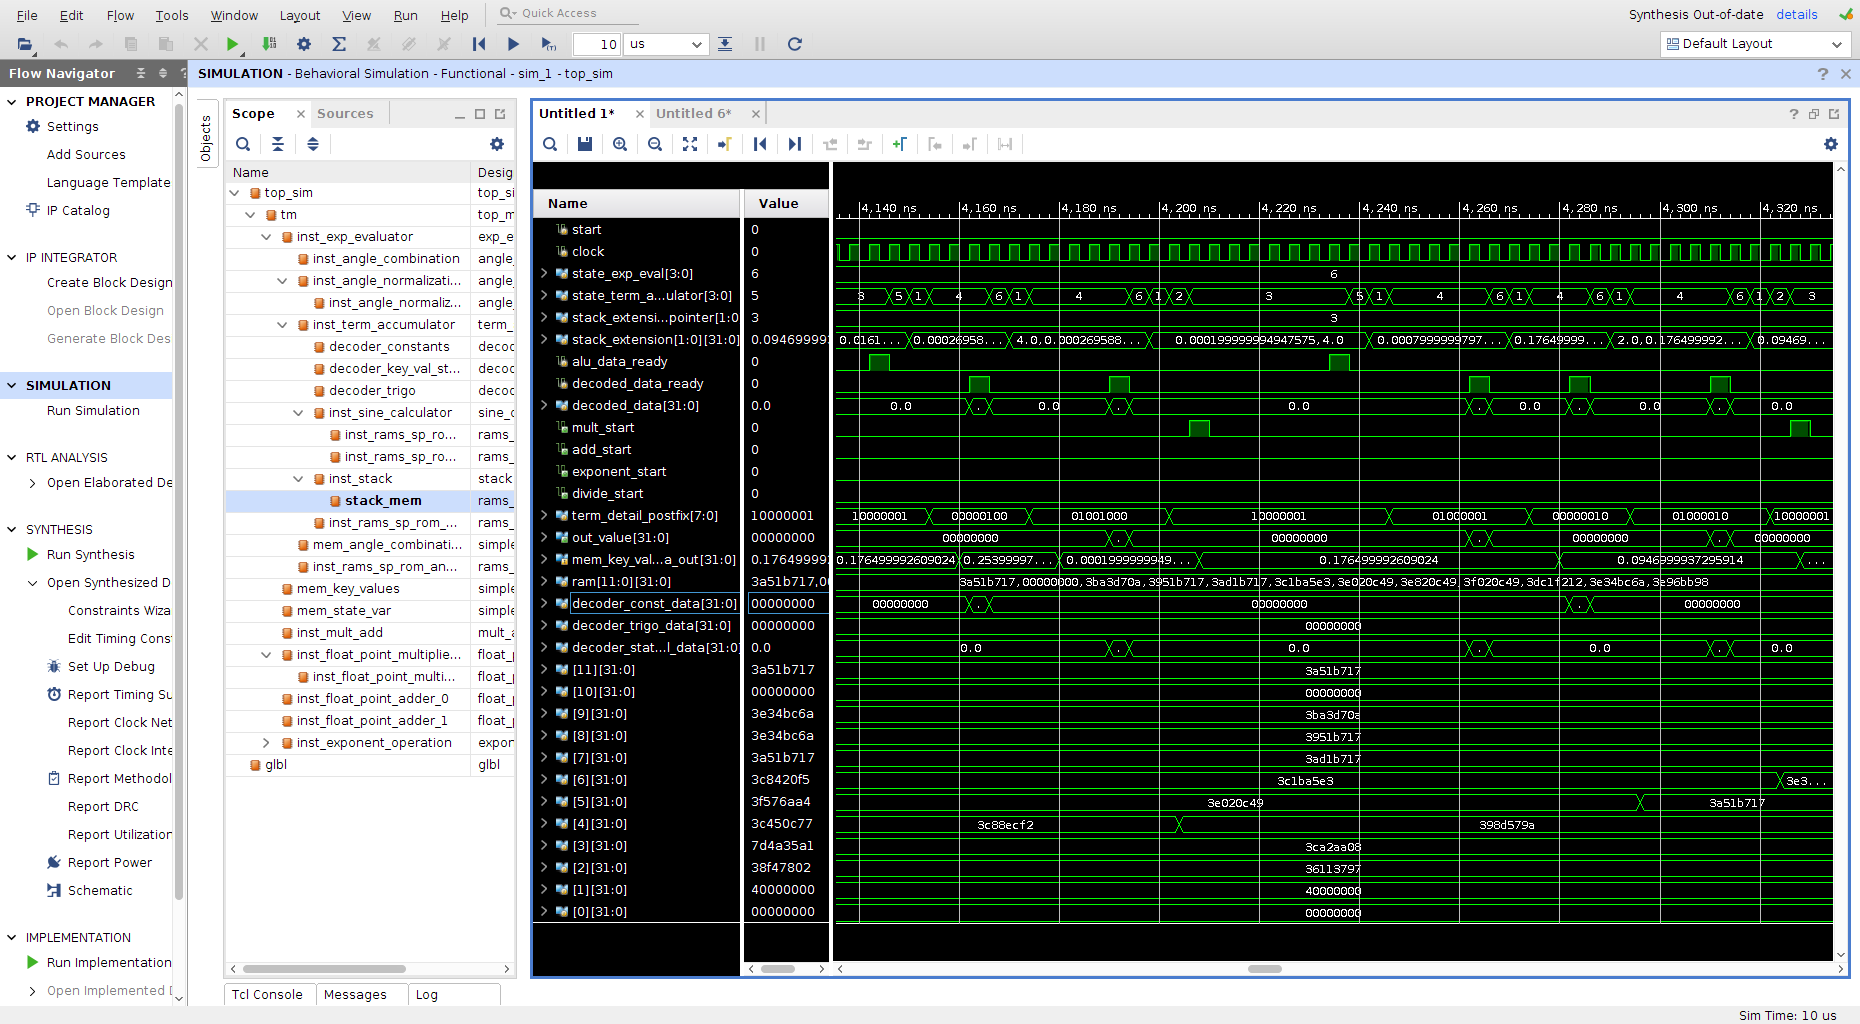
\includegraphics[width=16cm]{vivado_simulation.png}
\caption{Simulation of hardware implementation  in Xilinx Vivado}\label{fig:vivado_simulation}
\end{figure}

From the analysis presented in section 5.5 and the results obtained from the hardware simulation of the FPGA implementation, we can conclude that this design can serve as a good prototype of a chaos based cryptographic hardware which is immune against brute force quantum computing attacks.
        % Chapter 6: Finally the summary & conclusions
\chapter{Future Work}
\label{chap:future}
\setlength{\parskip}{1.5mm}
%\setlength{\baselineskip}{1.4mm}
This report so far discussed the methods for encryption-decryption based on non-linear chaotic map and its utility in post-quantum cryptography. Through a number of simulations, we can conclude that this cryptosystem can provide the desired level of chaos and security. Moreover, this cryptosystem also fulfills the basic requirements of a cryptosystem defined by Shannon including diffusion and confusion.
\subsubsection{Algorithmic Aspect}
The main improvement aspect of this work lies in the extension of this algorithm for asymmetric key cryptography. This can be easily done by introducing safe key manipulation techniques which would enable both parties to retrieve the key values. Once the key is obtained, one can proceed according to steps followed for the symmetric algorithm. Another improvement is introducing permutation map between characters and Baptista type partitioned intervals. Also instead of taking a single state variable value for chaotic map, all three state variable values can be combined through a one-one function to give a better level of encryption. For better validation of the cryptosystem in regards to the quantum-computing aspect, the cryptosystem must be tested against practical quantum computing algorithms for breaking cryptosystems which is beyond our current scope. However, this cryptosystem might serve well  practically in terms of both speed and cost.

\subsubsection{Hardware Implementation Aspect}
Although a complete implementation of the cryptographic algorithm has been presented, there remains a huge scope for improvement. This involves efficient caching of results of operations on constants. Implementation of such a cache can result in significant reduction in the number of clock cycles required. Furthermore, few modifications might be made to enable design scale easily according to the amount of resources at disposal.
             % Chapter 5: Simulation and Results


%=====================================================================
% APPENDIX
%  Appendices, if any, must precede the cited literatures.
%  Appendices shall be numbered in Roman Capitals (e.g. Appendix IV)

%% \appendix
%% \include{appendix_something}

%=====================================================================
% BIBLIOGRAPHY
%   This should follow the appendices, if any, otherwise summary and
%   conclusions chapter.
% Choose your bibliography style
% plain is the basic style, others include ieeetr, siam, asm, etc
%\bibliographystyle{plain}
% Add the bib file
%% \bibliography{bibfile}
\begin{thebibliography}{11}
\begin{small}

\bibitem{ref:habutsu}
Toshiki Habutsu, Yoshifumi Nishio, Iwao Sasase, Shinsaku Mori, ``A Secret Key Cryptosystem by Iterating a Chaotic Map'', {\em LNCS, vol 547}, EUROCRYPT 1991.

\bibitem{ref:yang}
T. Yang, ``A survey of chaotic secure communication systems'', {\em Int. J. Comput. Cogn. 2004}.

\bibitem{ref:hasler}
M. Hasler, ``Synchronization of chaotic systems and transmission of information'', {\em Int. J. Bifursc. Chaos, vol. 8, no. 4, Apr. 1998}.

\bibitem{ref:kocarev}
Ljupco Kocarev, ``Chaos-Based Cryptography: A Brief Overview'', {\em IEEE Circuits and Systems Magazine 1(3):6 - 21 , Sept 2002}.

\bibitem{ref:schmitz}
R. Schmitz, ``Symmetric ciphers based on two-dimensional chaotic maps'', {\em J. Franklin Inst., vol. 338, pp. 429-441, 2001}.

\bibitem{ref:knuth}
D. E. Knuth, ``The Art of Computer Programming.'', {\em MA: Addison-Wesley, 1998, vol. 2}.

\bibitem{ref:amigo}
L. Kocarev, J. Szczepanski, J. M. Amigo, and I. Tomosvski, ``Chaos-based Cryptography: an overview'', {\em International Symposium on Nonlinear Theory and its Applications (NOLTA2005), Bruges, Belgium, October 18-21, 2005.
}

\bibitem{ref:mathews}
R. Matthews, D. Wheeler, ``Supercomputer investigations of a chaotic encryption algorithm'', {\em Cryptologia XV, (1991) 140-152}.

\bibitem{ref:eyre}
Zbigniew Kotulski, Janusz Szczepanski, ``Discrete chaotic cryptography'', {\em Ann. Physik 6 (1997) 381-394}

\bibitem{ref:wichert}
Sofia Wichert, Konstantinos Fokianos and Korbinian Strimmer, ``Identifying periodically expressed transcripts in microarray time series data'', {\em Bioinformatics. 20 1, (2004), 5-20}.

\bibitem{ref:bernstein}
Daniel J. Bernstein, Johannes Buchmann, Erik Dahmen, ``Post-Quantum Cryptography''{\em Springer, Berlin, 2009}.

\bibitem{ref:lone}
Peter W. Shor, ``Polynomial-Time Algorithms for Prime Factorization and Discrete Logarithms on a Quantum Computer'', {\em SIAM J.Sci.Statist.Comput. 26 (1997) 1484}

\bibitem{ref:botha}
Andre E. Botha,Guoyuan Qi, ``Analysis of the Triple Pendulum as a
Hyperchaotic System''{\em Chaotic Modeling and Simulation (CMSIM) 2: 297{304, 2013}.}

\bibitem{ref:li}
Shujun Li, Guanrong Chen, Kwok-Wo Wong, Xuanqin Mou, Yuanlong Cai, ``Baptista-type chaotic cryptosystems: Problems and countermeasures'', {\em Physics Letters A, 332(5-6):368-375, 2004}

\bibitem{ref:lone}
Auqib Hamid Lone, Prof. Moin Uddin, ``Common Attacks on RSA and its Variants with Possible Countermeasures'', {\em International Journal of
Emerging Research in Management \& Technology
ISSN: 2278-9359 (Volume-5, Issue-5), May 2016}


\end{small}
\end{thebibliography}
%=====================================================================
% PUBLICATIONS
%  publications if any may be listed after the literature cited.
%% \include{mypubs}

%=====================================================================


\end{document} 
